\section{Verteilung}
\subsection{Effizienz}
Pareto-Effizienz: Eine wirtschaftspolitische Massnahme ist dann effizient wenn sie die Situation eines Einzelnen verbessert, ohne andere schlechter zu stellen. 
\subsection{Verteilung}
\begin{itemize}
	\item Die Einkommensverteilung hängt ab von der Produktivität der Arbeitenden.
	\item Daher verdienen weniger leistungsfähige wenig.
	\item Will die Gesellschaft dies nicht akzeptieren, so muss umverteilt werden.
	\item Wird zu viel umverteilt gibt es weniger Anreize zur persönlichen Leistung.
	\item Wird zu wenig umverteilt wird dies als ungerecht empfunden.
	\item Die Herausforderung ist die Verteilung mit möglichst geringen Anreizen zur Verschwendung von Ressourcen zu erreichen
	\item Gini-Koeffizient sagt nichts über Wohlstand aus, sondern nur über die Einkommensverteilung
\end{itemize}
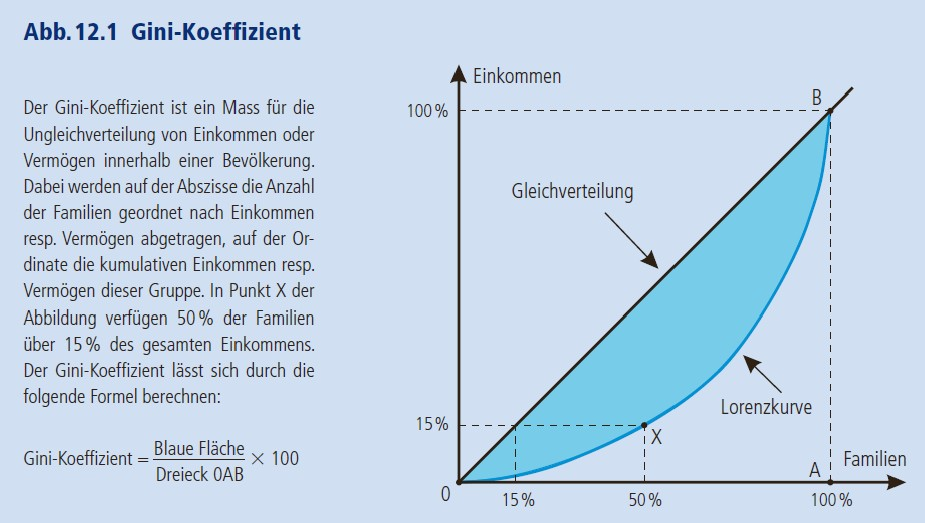
\includegraphics[width=0.7\linewidth]{images/gini.jpg}
\subsection{Umverteilung} 
\begin{minipage}{5cm}
	\textbf{Einkommensquellen}
	\begin{itemize}
		\item Lohn
		\item Erträge aus Vermögen
		\item Staatliche Transfers
	\end{itemize}
\end{minipage}
\begin{minipage}{15cm}
	\textbf{Arten der Umverteilung}
	\begin{itemize}
		\item Umverteilung Einnahmen durch progressives Steuersystem (Einnahmeseite)
		\item Direkte Geldzahlungen (Ausgabeseite)
		\item Verbilligung staatliche Leistungen (Ausgabeseite)
	\end{itemize}
\end{minipage}
\clearpage
\pagebreak
\subsection{Umverteilung Ausgabenseite: Sozialwerke}
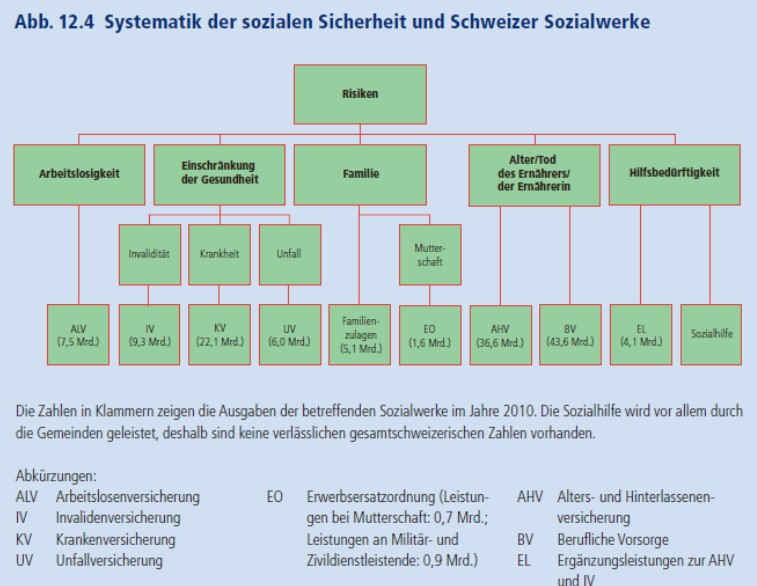
\includegraphics[width=0.8\linewidth]{images/sozialwerke.jpg}
\subsection{Die drei Säulen der Altersvorsorge der Schweiz}
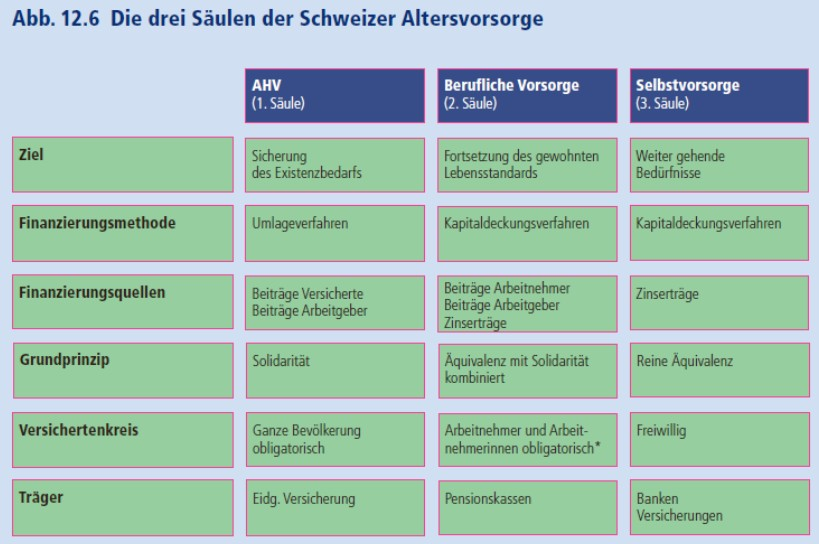
\includegraphics[width=0.8\linewidth]{images/dreisaulen.jpg}
\clearpage
\pagebreak